\documentclass{article}

\usepackage[utf8]{inputenc}
\usepackage[T1]{fontenc}
\usepackage[brazil]{babel}
\usepackage{amsmath}
\usepackage{booktabs}
\usepackage{graphicx}
\usepackage{hyperref}

\title{Cinemática do Robô Franka Emika Panda}
\author{Prof. Glauber R. Leite}
\date{Maio de 2026}

\begin{document}

\maketitle

\section{Apresentação do robô}

O robô utilizado neste projeto é o Franka Emika Panda, um manipulador serial
redundante com sete juntas rotacionais. Por possuir sete graus de liberdade, o
robô consegue posicionar e orientar o efetuador final no espaço tridimensional
mantendo uma liberdade adicional para evitar singularidades, contornar
obstáculos ou escolher posturas mais convenientes para a tarefa.

No projeto, o Franka é modelado e validado em simulação no CoppeliaSim. Os
scripts Python se conectam à cena por meio da API remota ZMQ, leem as posições
das juntas, calculam a cinemática direta, resolvem a cinemática inversa por
otimização e comparam os resultados com a pose do efetuador final obtida no
simulador.

\subsection{Descrição do espaço de configuração}

O espaço de configuração do Franka é definido pelo vetor

\[
q =
\begin{bmatrix}
q_1 & q_2 & q_3 & q_4 & q_5 & q_6 & q_7
\end{bmatrix}^{T},
\]

em que cada componente representa o ângulo de uma junta rotacional em radianos.
Neste trabalho são usados os limites articulares implementados no algoritmo de
cinemática inversa:

\[
\begin{aligned}
q_{\min} &=
\begin{bmatrix}
-2.8973 & -1.7628 & -2.8973 & -3.0718 & -2.8973 & 0.4363 & -3.0718
\end{bmatrix}^{T},\\
q_{\max} &=
\begin{bmatrix}
2.8973 & 1.7628 & 2.8973 & -0.0698 & 2.8973 & 4.6251 & 3.0718
\end{bmatrix}^{T}.
\end{aligned}
\]

\subsection{Cenários de aplicação}

Manipuladores redundantes como o Franka são usados em aplicações de pesquisa,
manipulação colaborativa, pick-and-place, inspeção, rastreamento de trajetórias
e tarefas que exigem movimentos suaves do efetuador final. A redundância é
especialmente útil quando há necessidade de atingir uma mesma pose cartesiana
com diferentes configurações articulares, permitindo escolher uma postura mais
segura ou mais distante de singularidades.

\section{Cinemática direta}

A cinemática direta foi descrita usando parâmetros de Denavit-Hartenberg
modificados, na convenção de Craig. Essa abordagem foi escolhida porque o
Franka é uma cadeia serial de juntas rotacionais e a representação DH permite
obter a transformação homogênea total pela multiplicação sequencial das
transformações entre elos.

Para cada junta, a transformação local usada no código é

\[
{}^{i-1}T_i =
\begin{bmatrix}
\cos\theta_i & -\sin\theta_i & 0 & a_{i-1}\\
\sin\theta_i\cos\alpha_{i-1} & \cos\theta_i\cos\alpha_{i-1} &
-\sin\alpha_{i-1} & -d_i\sin\alpha_{i-1}\\
\sin\theta_i\sin\alpha_{i-1} & \cos\theta_i\sin\alpha_{i-1} &
\cos\alpha_{i-1} & d_i\cos\alpha_{i-1}\\
0 & 0 & 0 & 1
\end{bmatrix}.
\]

A transformação homogênea global do efetuador final é

\[
{}^{0}T_{EE}(q) =
{}^{0}T_1
{}^{1}T_2
{}^{2}T_3
{}^{3}T_4
{}^{4}T_5
{}^{5}T_6
{}^{6}T_7
{}^{7}T_{EE}.
\]

\begin{table}[h]
\centering
\caption{Parâmetros DH modificados usados para o Franka}
\begin{tabular}{cccc}
\toprule
Elemento & $a_{i-1}$ (m) & $d_i$ (m) & $\alpha_{i-1}$ (rad)\\
\midrule
1 & 0 & 0.333 & 0\\
2 & 0 & 0 & $-\pi/2$\\
3 & 0 & 0.316 & $\pi/2$\\
4 & 0.0825 & 0 & $\pi/2$\\
5 & -0.0825 & 0.384 & $-\pi/2$\\
6 & 0 & 0 & $\pi/2$\\
7 & 0.088 & 0 & $\pi/2$\\
Efetuador & 0 & 0.107 & 0\\
\bottomrule
\end{tabular}
\end{table}

\begin{figure}[h]
    \centering
    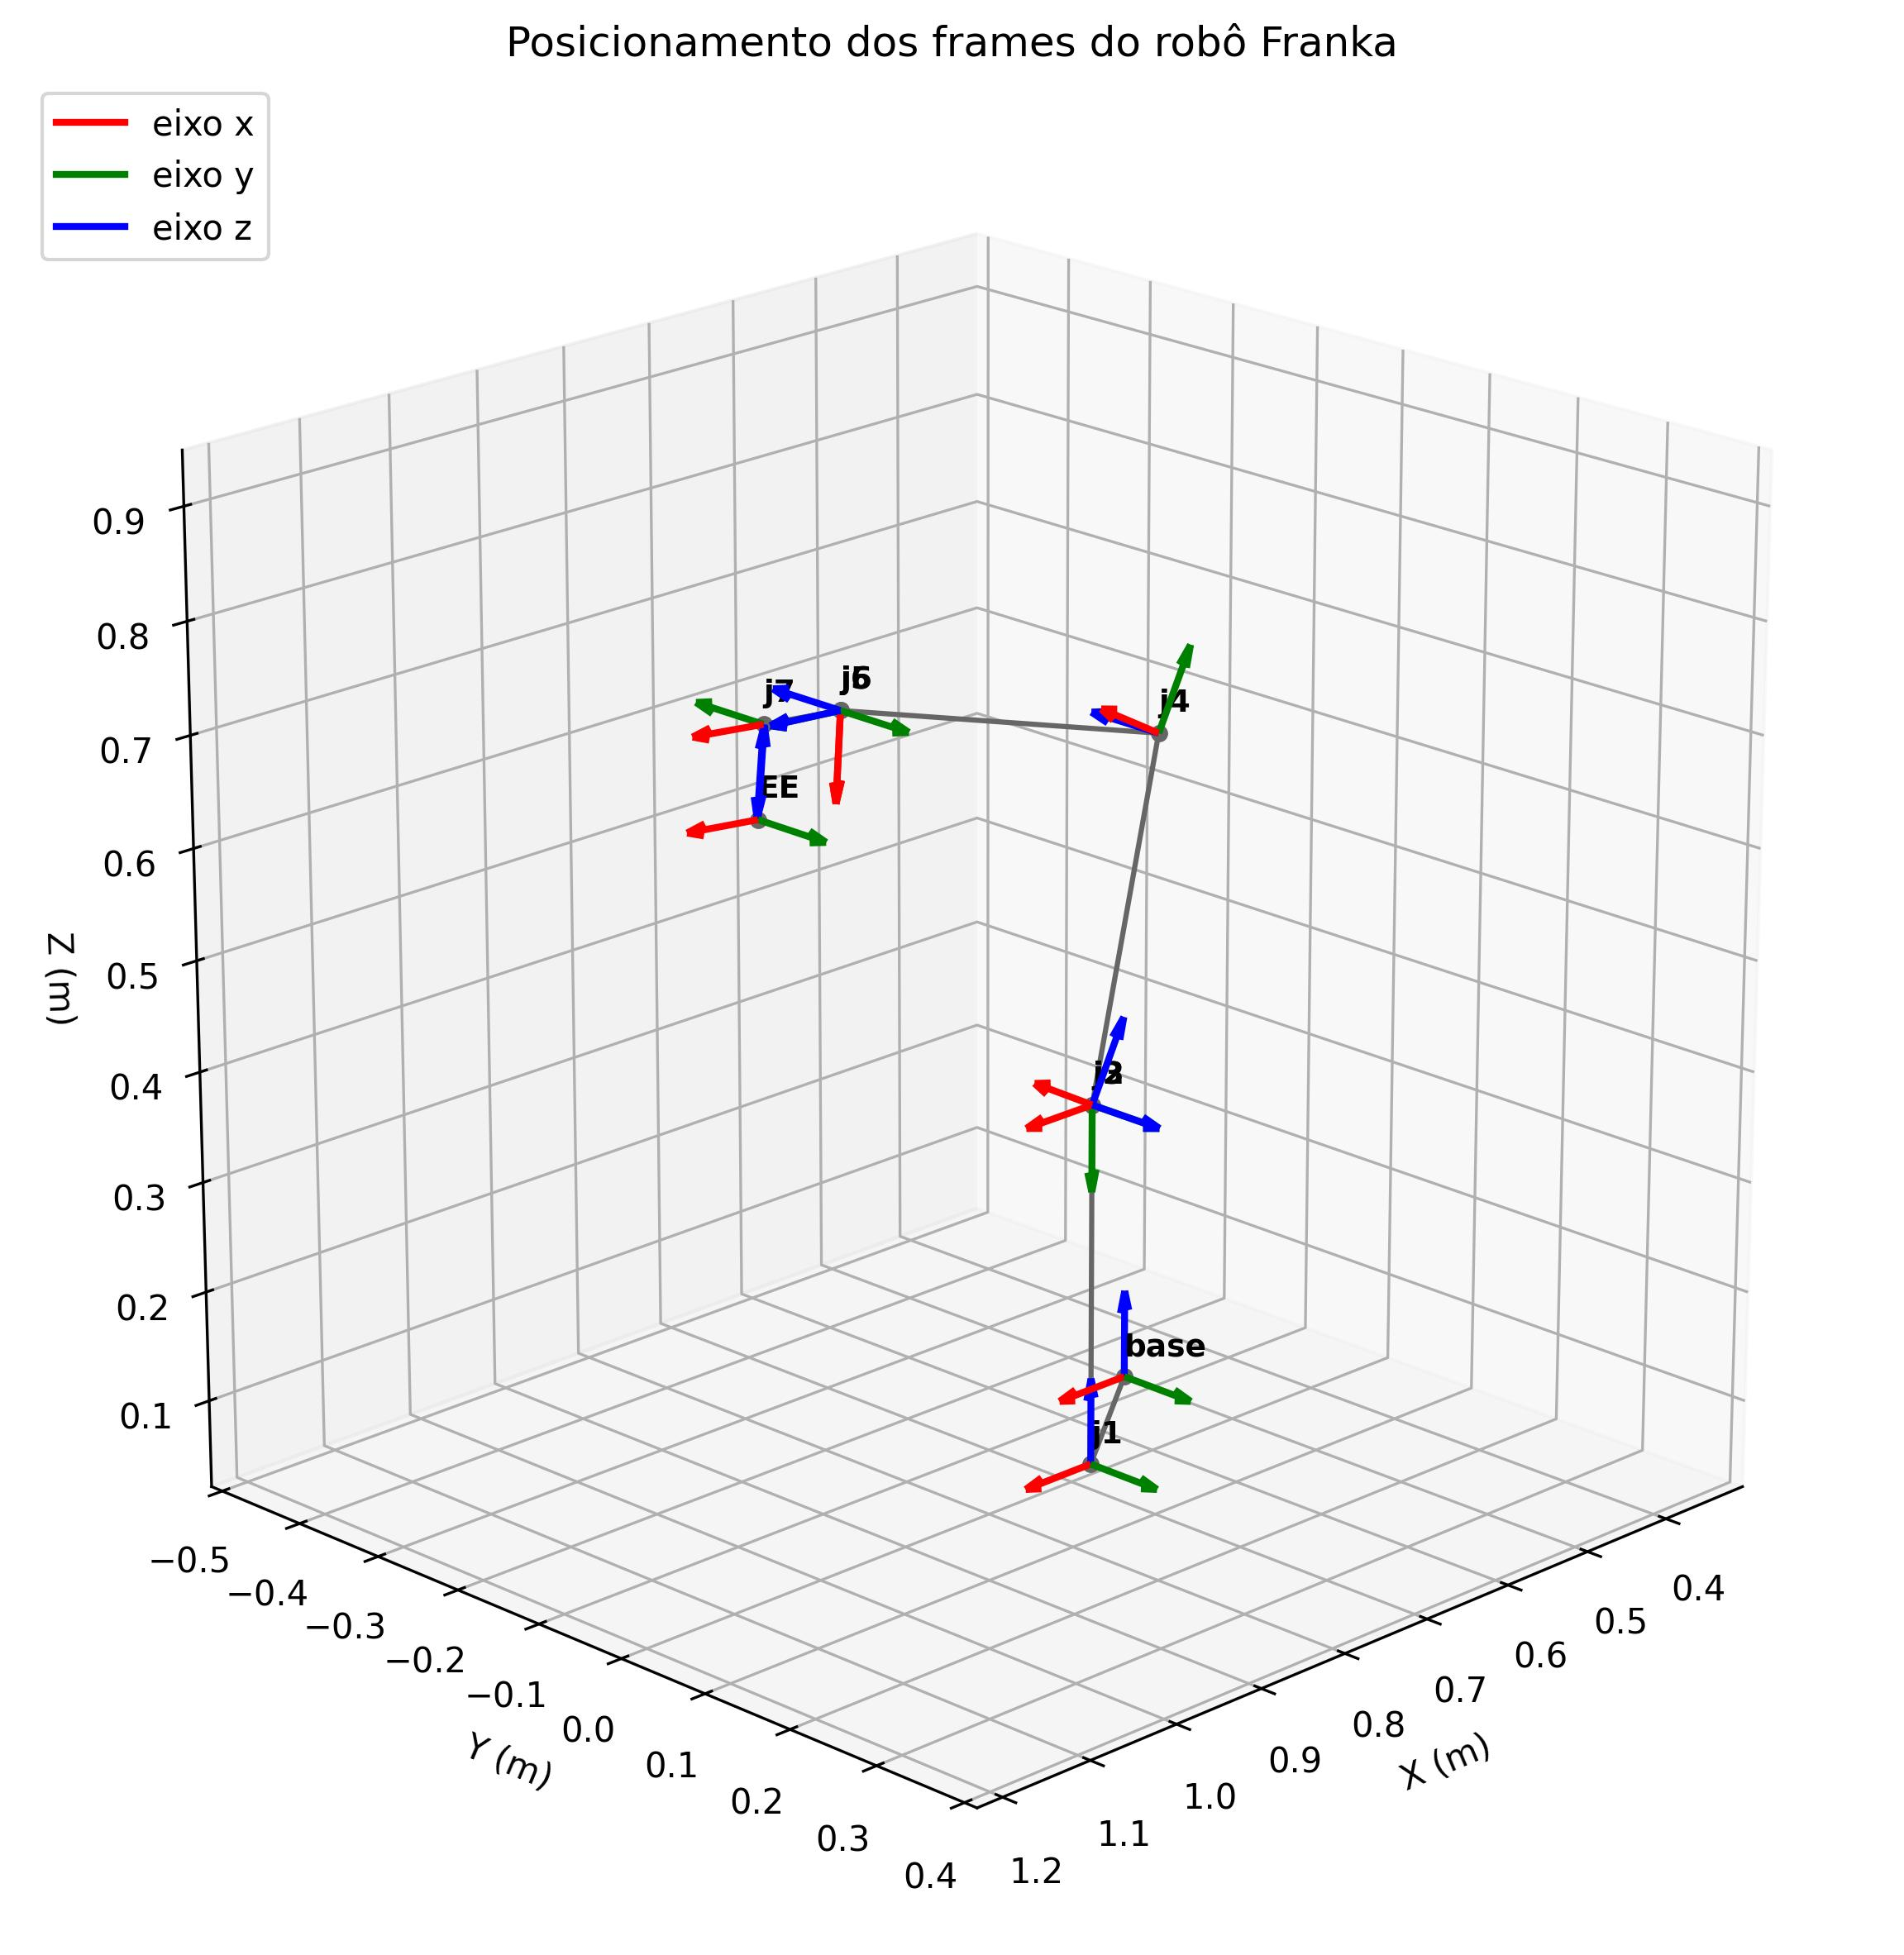
\includegraphics[width=0.9\linewidth]{franka_frames.jpg}
    \caption{Posicionamento dos frames do robô Franka}
    \label{fig:frames-franka}
\end{figure}

O script \texttt{cinematica\_franka.py} calcula a matriz homogênea total,
extrai a posição cartesiana do efetuador final e converte a matriz de rotação
para quatérnio no formato $(x,y,z,w)$. A pose calculada é comparada com a pose
obtida diretamente no CoppeliaSim para validar a modelagem.

\section{Cinemática inversa}

Como o Franka possui sete juntas para controlar a pose do efetuador final, a
cinemática inversa não tem solução única. Neste projeto, a solução foi tratada
como um problema de otimização não-linear com restrições de caixa nos limites
articulares.

O objetivo principal é minimizar o erro entre a posição calculada pela
cinemática direta e a posição alvo. Além disso, é adicionada uma penalização de
postura para favorecer uma configuração de referência segura:

\[
q_{\mathrm{ref}} =
\begin{bmatrix}
0 & -0.5 & 0 & -2.0 & 0 & 1.6 & 0
\end{bmatrix}^{T}.
\]

O vetor de resíduos minimizado pelo algoritmo é

\[
r(q) =
\begin{bmatrix}
k_p\left(p_{FK}(q) - p_{\mathrm{alvo}}\right)\\
W\left(q - q_{\mathrm{ref}}\right)
\end{bmatrix},
\]

em que $p_{FK}(q)$ é a posição do efetuador obtida pela cinemática direta,
$p_{\mathrm{alvo}}$ é a posição desejada, $k_p = 5$ é o peso do erro de posição
e $W$ é uma matriz diagonal de pesos articulares. O problema resolvido é

\[
\min_{q} \|r(q)\|^2
\quad
\text{sujeito a}
\quad
q_{\min} \leq q \leq q_{\max}.
\]

O script \texttt{inversa.py} resolve esse problema usando o método
\textit{Trust Region Reflective}, implementado em \texttt{scipy.optimize.least\_squares}.
Quando há uma cena ativa no CoppeliaSim, o alvo pode ser lido a partir de um
objeto chamado \texttt{/Cuboid}; caso contrário, o módulo também pode ser usado
em testes offline para recuperar uma configuração a partir de uma posição
gerada pela própria cinemática direta.

\section{Arquivos do projeto}

\begin{itemize}
    \item \texttt{cinematica\_franka.py}: implementação da cinemática direta e validação contra o CoppeliaSim.
    \item \texttt{inversa.py}: implementação da cinemática inversa por otimização.
    \item \texttt{pose.py}: geração da figura com os frames do robô.
    \item \texttt{poses\_franka.py}: execução de uma sequência de poses articulares no CoppeliaSim.
    \item \texttt{pick\_and\_place\_franka.py}: tarefa simulada de pegar um cubo, transportar por waypoints e soltar em outro ponto.
    \item \texttt{pick\_and\_place\_obstaculos\_franka.py}: extensão do pick-and-place com obstáculos, desvio por waypoints cartesianos, registro da trajetória executada e métricas de desempenho.
    \item \texttt{pick\_and\_place\_complexo\_franka.py}: processo em duas etapas com coleta, inspeção intermediária, nova coleta, entrega final, obstáculos, métricas e gráficos.
    \item \texttt{pick\_and\_place\_sorting\_franka.py}: célula de classificação com três peças coloridas, inspeção intermediária, destinos diferentes, obstáculos, métricas e gráficos.
    \item \texttt{teste-copellia.py}: teste de movimentação articular no CoppeliaSim.
    \item \texttt{ate\_o\_cubo.py}: exemplo de movimento do efetuador final até um cubo na cena.
\end{itemize}

\end{document}
